\documentclass{IEEEtran}

\usepackage{amsmath}
\usepackage{listings}
\lstset{
    basicstyle=\small\ttfamily,
    breaklines=true
}
\usepackage{graphicx}
\graphicspath{ {./images/} }

\title{Readings about DP on Trees}
\author{Diego Linares - kiwiAipom}

\begin{document}
    \maketitle

    \section{DP on Trees Tutorial}
        Pre-requisites for the reading:
        \begin{itemize}
            \item Basic dynamic programming: optimal substructure property and memoisation.
            \item Trees (basic DFS, subtree definition, children, etc.)
        \end{itemize}
        \textbf{DP definition:} solve problems by breaking them down into overlapping sub-problems which follow the optimal substructure.\\
        We define functions for nodes, which we calculate recursively based on children of a node. One of the states of the \textbf{DP} usually is a node $i$, so we are solving for its subtree.
        \subsection{Problem 1}
            Tree $T$ with $N$ nodes, each node $i$ has $C_i$ coins attached to it. Choose a subset of nodes such as no two nodes are \textit{adjacent}, and the sum of coins is max.\\
            A similar problem was for an $A = \{a_1,a_2,\ldots,a_n\}$. We chose $dp(i)$ as our answer for $a_1,a_2,\ldots,a_i$. The recurrence being $dp(i) = max(a_i+dp(i-2),dp(i-1))$ (choose $a_i$ or not, basically).\\
            In a tree first we need to root it. For example at node $1$ and define $dp(V)$ as the answer for subtree with root $V$, then $dp(1)$ is the answer.\\
            So if we include $V$ we can't include their children, but we can include any grandchildren.\\
            So the recurrency  of $dp(V)$ is: $$max(\sum_{i=1}^n dp(v_i), C_V + \sum_{i=1}^n\text{sum of $dp(j)$ for children $j$ of $v_i$})$$
            We can define two DP, $dp1(V), dp2(V)$, the first one is the number of coins that can be obtained from the subtree, and the second one, if we include the node or not. Final answer being $max(dp1(1) + dp2(1))$\\
            Now the recursion is easier: $$dp1(V) = C_V + \sum_{i=1}^ndp2(v_i)$$
            Since the answer of a node is dependent on the one of its children, we need a recursive DFS implementation.
            \begin{lstlisting}
vector<int> adj[N] // contains all neighbors of i node.
int dp1[N], dp[2]; 
void dfs(int V, int pV) // pV is the parent of node V
{
    // for storing sums of dp1 and max(dp1,dp2) for all children of V
    int sum1 = 0, sum2 = 0; 
    // traverse over all children
    for (auto v: adj[V])
    {
        if (v == pV) continue;
        dfs(v,V);
        sum1 += dp2[v];
        sum2 += max(dp1[v], dp2[v]);
    }
    dp1[V] = C[V] + sum1;
    dp2[V] = sum2; 
}
int main()
{
    int n;
    cin >> n;
    for(int i=1; i<n; i++)
    {
        cin >> u >> v;
        adj[u].push_back(v);
        adj[v].push_back(u);
    }
    dfs(1,0); // this basically does the DFS for all the nodes.
    int ans =  max(dp1[1], dp2[1]);
    cout << ans << endl; 
}
            \end{lstlisting}
            Complexity: $O(N)$.
        \subsection{Problem 2}
            Given a tree $T$ of $N$ nodes, longest path between two nodes (\textit{diameter of the tree}). If we root node 1, there exists a node $x$ such that:
            \begin{itemize}
                \item Longest path starts from node $x$ and goes into the subtree. Denote this as $f(x)$. Blue
                \item Starts in the subtree of $x$, passes through it, and then back into the subtree. Denote this as $g(x)$. Red. 
            \end{itemize}
            \begin{center}
                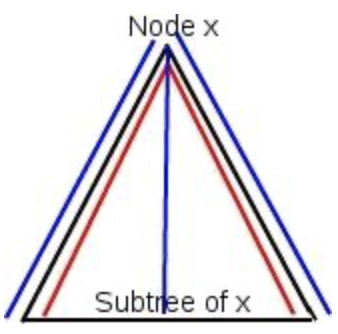
\includegraphics[width=0.13\textwidth]{dpTreeNodeX.png}
            \end{center}
            If we get the max from both for all nodes $x$ we can calculate the diameter, but how can we calculate max path length in both cases?\\
            A node $V$ has $n$ children $v_1\ldots v_n$. $f(i)$ is the length of longest path that starts at node $i$ and ends in its sub tree. So $f(V) = 1 + max(f(v_1),\ldots,f(v_n))$. Since it is the maximum path of their children, plus the father.\\
            \textit{As you can see in DP on trees functions are for nodes and recursion is based on values of children}.\\
            Case 2: originate from subtree of $v_i$, go through $V$ and end in the subtree of $v_j$, where $i\neq j$. To make the path maximum we'll make $f(v_i), f(v_j)$ to be maximum. So $g(V) = 1 + \text{ sum of two max from set } \{f(v_1),\ldots,f(v_n)\}$.\\
            We calculate $f$ through a DFS and on the go. It's done in $O(N)$
            \begin{lstlisting}
vector<int> adj[N];
int f[N],g[N], diameter;
void(int V, int pV)
{
    vector<int> fValues; // f for all children of V
    for(auto v: adj[V])
    {
        if(v == pV) continue;
        dfs(v,V);
        fValues.push_back(f[v]);
    }
    //Sort to get the two biggest values
    sort(fValues.begin(),fValues.end());
    f[V] = 1; // update for the current node
    if(!fValues.empty()) f[V] += fValues.back();
    if(fValues.size() >= 2) // more than 2 kids
        g[V] = 2 + fValues.back() + fValues[fValues.size()-2]; // the two biggest.
    diameter = max(diameter, max(f[V],g[V]));
}
            \end{lstlisting}
        \subsection{Problem 3}
            Tree $T$ with $N$ nodes. Find number of \textbf{sub trees} of size $\leq K$.\\
            \textbf{Sub Tree (separated):} connected subset of nodes from the original tree.\\
            Suppose the tree is rooted at 1, $S(V)$ is the subtree rooted at node $V$ (different definition from the one in the problem), since all the nodes are included.\\
            \textbf{How to count the number of sub trees of a tree?} We define $f(V)$ as the number of sub trees of $S(V)$ (subtree with the node included). So for each child $u$ of $V$ we have the choice of including them in the sub tree (which there are $f(u)$ ways of doing) or not (just 1 way, because we wont choose its children).\\
            Node $V$ has children $v_1,\ldots,v_n$, so $f(V) = \prod_{i=1}^n 1 + f(v_i)$ (el producto del f de cada uno de los hijos). That function considers the subtrees \textbf{rooted} at $V$. We now define $g(V)$ for the ones not rooted at $V$, its recursion being:
            $$\sum_{i=1}^n f(i)+g(i)$$
            For each child we add to $g(V)$ number of ways to choose a subtree rooted or not at that child. So the final answer is $f(1) + g(1)$ (for this partial problem).\\
            \textbf{How many of these don't exceed $K$ size?} We add another state to the $dp, f(V,k)$ being the number of sub trees with $k$ nodes and $V$ as root. If a child $S(v_i)$ contributes $a_i$ nodes, $k$ is $\sum_{i=1}^n a_i$. If we want to form a sub tree of size $k+1$ (one node contributed by $V$), $f(V,k)$ is the sum of $\prod_{i=1}^n f(v_i,a_i)$ for all distinct sequences $a_1,\ldots,a_n$.\\
            How to compute this? $dp1(i,j)$ is the way to choose $j$ nodes from subtrees $v_1,\ldots,v_i$, and its recurrence is: $dp1(i,j)=\sum_{k=0}^K dp1(i-1,j-k)*f(i,k)$ (iteratiing over $k$ assuming that subtree of $v_i$ contains $k$ nodes). Finally:
            $$f(V,k) = dp1(n,k)$$
            $$\sum_{i=1}^K f(V,i) \text{ for all nodes } V$$
            In pseudo-code:
            \begin{lstlisting}
f[N][K+1]; // K+1 since you will include 0
void rec(int cur_node)
{
    f[cur_node][1] = 1
    dp_buffer[K] = {0}
    dp_buffer[0] = 1

    for(all v such that v is children of cur_node)
        rec(v)
        dp_buffer1[K] = {0}
        for i = 0 to K:
            for j = 0 to K - i:
                dp_buffer1[i+j] += dp_buffer[i]*f[v][j]
        dp_buffer = dp_buffer1
    f[cur_node] = dp_buffer
}
            \end{lstlisting}
            Complexity: $n$ children, so $O(N*K^2)$\\
            A similar problem: $N$ nodeds and weight of each, delete enough nodes so it has $K$ leaves. Cost is the weight of the node. Try to find the minimum cost. (\textit{check Indian Computing Olympiad})
        \subsection{Problem 4}
            Each node $i$ has a cost $C_i$. Start in root, choose unvisited node at random until there are no unvisited. Cost of travel is the sum of costs so far. \textit{Which node should be the root?}\\
            $f(V)$ is expected total time if we start at node $V$ and visit in its subtree.
            $$f(V) = C_V + \frac{\sum_{i=1}^n f(v_i)}{n}$$
            Now we find a node $v$ such that $f(v)$ is minimized. It depends on the root of the tree. Brute force is too slow.\\
            \textbf{Idea:} Iterate over all nodes $V$ and calculate the value of $f(V)$ if the tree is rooted at it. \textit{We need to see the contribution of $f(parent(V))$ if tree is rooted at $V$}. $g(V)$ is defined as the expected total time at $parent(V)$, if we don't consider the contribution of the subtree of $V$.\\
            Total expected time now is:
            $$C_V = \frac{g(V) + \sum_{i=1}^n f(v_i)}{n+1}$$
            To calculate $g(V)$ consiedr a node $p$ with parent $p'$ and children $v_1,\ldots,v_n$. To find $g(v_i)$, which means root tree at nodee $p$ and \textbf{don't consider} subtree of $v_i$ for calculating $f(p)$.
            $$C_p+\frac{g(p)+f(v_i)+\ldots+f(v_{i-1})+f(v_{i+1})+\ldots+f(v_n)}{n}$$
            $g(p)$ gives us the time at  $p'$ without considering the subtree of $`$. And we divide by the $n$ since it is the number of adjacent nodes of $p$, minus the one we are not considering.\\
            \begin{center}
                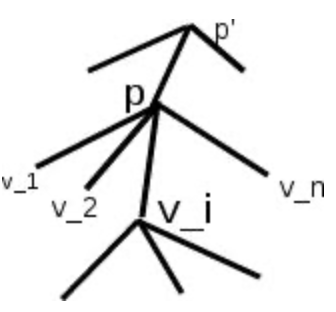
\includegraphics[width = 0.15\textwidth]{randomTreeDP.png}
            \end{center}
            $f,g$ can be calculated recursively in $O(N)$.
        \subsection{Problem 5}
            You have to make $T_1$ as structurally similar to $T_2$ which can be done by inserting leaves in any of the trees. Minimum number of insertions to do so.\\
            Suppose both are rooted at $1$. $T_{1_1}$ with children $u_1,\ldots,u_n$ and $T_{2_1}$ with $v_1,\ldots,v_m$- We map nodes between sets, making $u_i = v_j$ in terms of structure, for some $i,j$, by addding the required nodes. If $n\neq m$ we add the whole subtree required.\\
            \textbf{How to choose which node to map?} $dp(i,j)$ is the minimum additions required to make the subtree of $i$ to the one of $j$.\\
            So we gonna assign a node $u_i$ to $v_j$, the cost gonna be $dp(u_i,v_j)$. We have to assign such that the cost is minimized, \textbf{assignment problem}. Cost matrix $C$ in which $C(i,j)$ is the cost of assigning $i$ to $j$. Solving this matrix can be done in $O(N^3)$, if there are $N$ tasks. $C(i,j) = dp(u_i,v_j)$ so we can get $dp(i,j)$.\\
            Complexity ends up being $O(N^3)$, $N$ being the maximum number of nodes between the trees.
        
    \section{Another DP on Trees Tutorial}
        \subsection{Lowest Common Ancestor}
            This technique is known as \textbf{binary lifting.} It allows you to find the LCA in $\lg{n}$. Basically the lowest node that serves as root for the subtree that includes both nodes.\\
            So while we are doing \textit{I am pretty sure he said DFS}, we can obtain the depth of $L[\mu]$ ($\mu$ being a node), which is equal to $1+L[parent]$. Now let us create the following:
            $$p[\mu][0]=parent$$
            $p$ is a 2d array of space $n\lg{n}$. Where $p[\mu][i]$ means the ancester of $\mu$, $2^i$ steps up. So suppose that $x = P[\mu][i]$, then $P[\mu][i+1] = P[x][i]$.\\
            We can get $P[\mu][0]$ for all $\mu$, and then we can get the rest of the array easily in $n\lg{n}$. Having $N$ values of $\mu$ and $\lg{n}$ values of $i$.\\
            So, suppose that you have nodes $u,v$, suppose \textit{without loss of generalization} that $L[u] \geq L[v]$ (if not you can "swap" which one is your $u,v$ to achieve this). Move from $u$ upwards until you reach the node $x$ that is the same level as $v$.\\
            So suppose the difference between $L[v]$ and $L[u]$ is $Z$, how do we know how to jump towards it in $\lg{n}$ time. The steps are:
            \begin{enumerate}
                \item Take the greatest factor of $2$ that is $\leq Z$
                \item Jumpthose many steps
                \item Substract that from $Z$
                \item Go to step one again. Until $Z=0$s
            \end{enumerate}
            So now we have 2 cases:
            \begin{enumerate}
                \item $u = v$ which happens when $v$ is an ancestor of $u$. In this case just return $v$
                \item They are not equal, but they are now at the same level. So we can take the distance to their common ancestor as $Y$. Though we don't know its value
            \end{enumerate}
            Let's have an $i$ which iterates from the highest power of 2 towards 1. If $P[u][i] \neq P[v][i]$, I move both nodes $i$ steps upwards. Keep doing this an you will eventually arrive to the point where the common ancestor is their parent. Then simply return $P[u][0]$.\\
            \begin{center}
                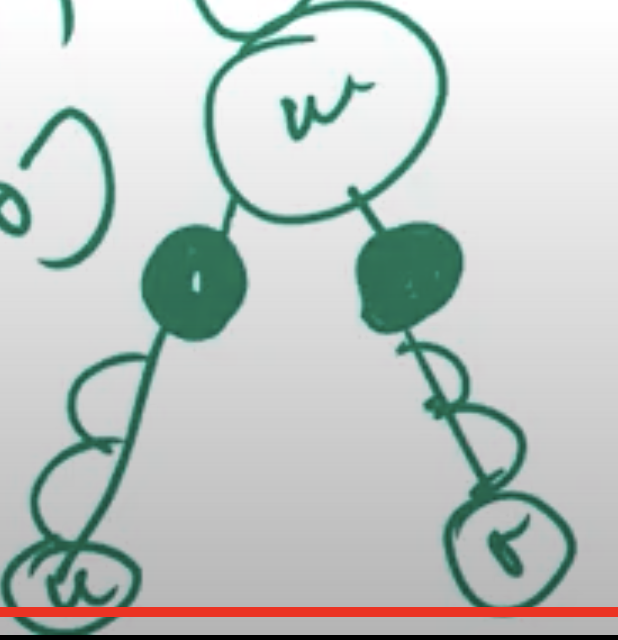
\includegraphics[width=0.15\textwidth]{lcaExample.png}
            \end{center}
            \subsubsection{Example: Distance between u and v} 
                It's easy. Compute the tree, then find the LCA of $u,v$ which we will not as $w$ and then the distance would be:
                $$L[u]+L[v]-2L[w]$$
            \subsubsection{Implementation}
                This is the code for the $dfs$ function which get us the levels. We start with $1,0$ as parameters.
                \begin{lstlisting}
void dfs(int u, int par)
{
    L[u] = 1 + L[par];
    P[u][0] = par;
        for(int v:g[u])
        {
            if (v == par) continue;
            dfs(v, u);
        }
}
                \end{lstlisting}
                And the code for the LCA is the following:
                \begin{lstlisting}
int lca(int u, int v)
{
    int i, lg;
    if(L[u] < L[v]) swap(u, v);
    for(lg = 0; (1<<lg) <= L[u]; lg++); // Finding the greatest power of 2
    lg--;
    if (u == v)
        return u;
    for(i = lg; i >= 0; i--)
    {
        if (P[u][i] != -1 and P[u][i] != P[v][i])
            u = P[u][i], v = P[v][i];
    }
    return P[u][0];
}
                \end{lstlisting}
                A few lines of code that I found interesting in the \texttt{main} were:
                \begin{lstlisting}
for(i = 1; i < LG; i++)
{
    Fo(j, 1, n+1) // A macro
        if(P[j][i-1] != -1)
            P[j][i] =P[P[j][i-1]][i-1];
}
                \end{lstlisting}
                Might come in handy.
        \subsection{Application in Competitive Programming}
            The problem we are going to solve is: \textit{Fafa and Ancient Mathematics} from Codeforces Round \#465 (Div.2).\\
            An \textit{Ahmed Arithmetic Expression (AAE)} is:
            \begin{itemize}
                \item "$d$", where $d$ is a one-digit positive integer.
                \item "$(E_1opE_2)$" where $E_1,E_2$ are AAE, and $op$ is $+,-$
            \end{itemize}
            You have an expression but don't know the operators. Find the max possible value after putting the operators in. You are given how many $+$ and $-$ operators there are.\\
            \textbf{Examples:}
            \begin{lstlisting}
Input:
    (1?1)
    1 0
Output: 2
Input: 
    (2?(1?2))
    1 1
Output: 1
            \end{lstlisting}
            In the tree that we are gonna make from the expression, \textbf{the leafs will be the digits}. Any non-leaf node will be a $?$ that will be filled with plus or minus. Each of them has 2 children which are the operands.\\
            The first thing we need to do is to build the tree, keeping in mind that the order of the operands matters ($2-3\neq 3-2$). So then:
            \begin{itemize}
                \item If the sign is $+$, we want the max value from the left and right operand.
                \item If the sign is $-$, we want the max value from the left and min from the right.
            \end{itemize}
            So let's take these 2 cases, and consider than in each we have $p$ plus signs, and $m$ minus signs. We have to consider all cases.\\
            \textbf{If we choose Plus} we will have $p - 1$ symbols to distribute between the left subtree (let's say $x$) and the right one ($p-1-x$). Knowing we have $count$ number of $?$ in the left subtree, then the number of minus symbols in the left subtree will be $count - x$. Something similar will happen in the right onw, which will have another value of $count$, and the amount of minus will be $count - (p-1-x)$.\\
            \textbf{If we choose Minus} Then we will have $max(x, count-x)$ on the left subtree, but in the right subtree we will go with $min(p-x, count-(p-x))$.\\
            So we will have to $DP$ states that we want to check. They will look like this:
            $$max(\mu,p,m)$$
            $$min(\mu,p,m)$$
            Now how do we minimize the value. Well, that depends on what value do we choose for the node $v$ again.\\
            \textbf{If we choose Plus} Then we shall try to minimize the value on the left side, and in the right side.\\
            \textbf{If we choose Minus} Then we shall try to minimize the value on the left side, and maximize the value on the right side.\\
            So basically we have 2 DP going on at the same time.\\
            By constraints we know that the value of $\mu$ can go all the way to $10^4$, and its value is defined by $count$, and since $m$ is defined by $count-p$ we \textbf{don't} need a third dimension for our $dp$. In fact, this value can be re-stated as $max(v,p)$ or $max(v,m)$ depending on if $p>m$ or otherwise.\\
            It's quite a long code, but fun to implement. \textit{Allegedly.}

    \section{Algorithms Lecture 1: Sums and Expected Value}

    \begin{thebibliography}{}
        \bibitem{mmi}
            \textit{DP on Trees Tutorial},
            darkshadow's blog,
            From: https://codeforces.com/blog/entry/20935
        \bibitem{rachi}
            \textit{Dynamic Programming on Trees}
            rachitiitr's blog,
            From: https://codeforces.com/blog/entry/61572
    \end{thebibliography}
\end{document}